\iffalse
\documentclass[journal,10pt,twocolumn]{article}
\usepackage{graphicx}
\graphicspath{{./Figures/}}
\usepackage[margin=0.5in]{geometry}
\usepackage[cmex10]{amsmath}
\usepackage{amssymb}
\usepackage{array}
\usepackage{booktabs}

\title{\textbf{Line Assignment}}
\author{Bole Manideep}
\date{September 2022}

\providecommand{\norm}[1]{\left\lVert#1\right\rVert}
\providecommand{\abs}[1]{\left\vert#1\right\vert}
\let\vec\mathbf
\newcommand{\myvec}[1]{\ensuremath{\begin{pmatrix}#1\end{pmatrix}}}
\newcommand{\mydet}[1]{\ensuremath{\begin{vmatrix}#1\end{vmatrix}}}
\providecommand{\brak}[1]{\ensuremath{\left(#1\right)}}

\begin{document}
\maketitle
\fi

	\begin{figure}[!h]
		\centering
 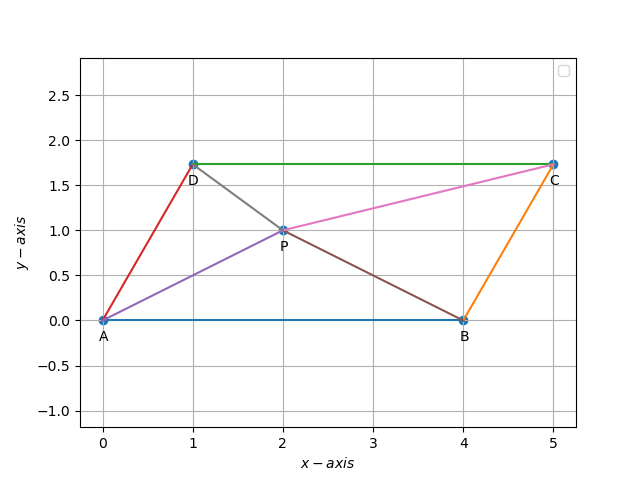
\includegraphics[width=\columnwidth]{chapters/9/9/2/4/figs/Question.png}
		\caption{}
		\label{fig:9/9/2/4}
  	\end{figure}
	\iffalse
\begin{figure}[h]
\centering
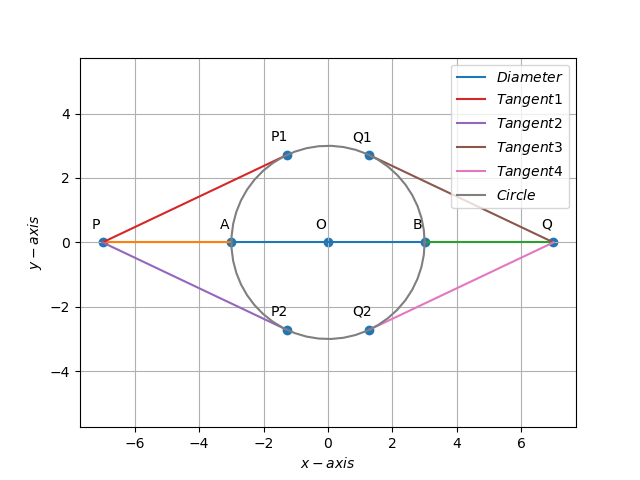
\includegraphics[width=1\columnwidth]{Question.png}
\caption{Parallelogram ABCD with interior point P}
\label{fig:Parallelogram}
\end{figure}

\section*{Solution}

\subsection*{Part 1}
WKT, area of a parallelogram with adjacent sides a \& b is,
\begin{equation}
\text{Area of parallelogram = } \norm{\vec{a} \times \vec{b}}
\label{eq-1-}
\end{equation}
And, area of a triangle with adjacent sides p \& q is,
\begin{equation}
\text{Area of triangle = } \frac{1}{2} \norm{\vec{p} \times \vec{q}}
\label{eq-2-}
\end{equation}
From Figure 1,\\ $\vec{(A-D)}\hspace{2mm}\&\hspace{2mm}\vec{(B-C)}$ are equal,\\
\begin{equation}
\norm{\vec{A-D}} = \norm{\vec{B-C}}
\label{eq-3-}
\end{equation}
Consider $\triangle$APD
\begin{equation}
\text{Area of } \triangle APD = \frac{1}{2}\norm{\vec{(A-D)} \times \vec{(A-P)}}
\label{eq-4-}
\end{equation}
Consider $\triangle$PBC
\begin{equation}
\text{Area of } \triangle BPC =  \frac{1}{2}\norm{\vec{(B-C)} \times \vec{(P-B)}}
\label{eq-5-}
\end{equation}
On adding \eqref{eq-4-} \& \eqref{eq-5-},
\begin{multline}
Ar(APD) + Ar(PBC) =\\
 \frac{1}{2}\norm{\vec{(A-D)} \times \vec{(A-P)}} + \frac{1}{2}\norm{\vec{(B-C)} \times \vec{(P-B)}}
\label{eq-6-}
\end{multline}
From equation \eqref{eq-3-},
\begin{multline}
Ar(APD) + Ar(PBC) =\\
 \frac{1}{2}\norm{\vec{(A-D)} \times \vec{(A-P)}} + \frac{1}{2}\norm{\vec{(A-D)} \times \vec{(P-B)}}
\label{eq-7-}
\end{multline}
\begin{multline}
\implies Ar(APD) + Ar(PBC) =\\ \frac{1}{2}\norm{\vec{(A-D)}\times[\vec{(A-P)} + \vec{(P-B)}]}
\label{eq-8-}
\end{multline}
Here, AP \& PB are adjacent sides of $\triangle$ APB
\\From Triangle law of vector addition, \\ $\vec{(A-P)} + \vec{(P-B)} = \vec{(A-B)}$
\begin{equation}
\implies Ar(APD) + Ar(PBC) = \frac{1}{2}\norm{\vec{(A-D)}\times\vec{(A-B)}}
\label{eq-9-}
\end{equation}
Since, $\vec{(A-D)} \hspace{2mm} \& \hspace{2mm} 1\vec{(A-B)}$ are adjacent sides of paralleogram ABCD
\\With reference to \eqref{eq-2-},
\begin{equation}
Ar(ABCD) = \norm{\vec{(A-D)}\times\vec{(A-B)}}
\label{eq-10-}
\end{equation}
From \eqref{eq-9-} \& \eqref{eq-10-}
\begin{equation}
\therefore \hspace{3mm} Ar(APD)+Ar(PBC) = \frac{1}{2}Ar(ABCD)
\label{eq-11-}
\end{equation}

\subsection*{Part 2}
Similarly, we can prove taht,
\begin{equation}
Ar(APB)+Ar(PBD) = \frac{1}{2}Ar(ABCD)
\label{eq-12-}
\end{equation}
On Comparing \eqref{eq-11-} and \eqref{eq-12-},
\begin{equation}
Ar(APD)+Ar(PBC) = Ar(APB)+Ar(PCD)
\label{eq-13-}
\end{equation}
\begin{center}
Hence Proved
\end{center}
\section*{Construction}
\raggedright A parallelogram ABCD is constructed unsing python,with the parameters that are mentioned in the table below.
\vspace{5mm}
\begin{center}
    \setlength{\arrayrulewidth}{0.1mm}
	\setlength{\tabcolsep}{12pt}
	\renewcommand{\arraystretch}{1.5}
\begin{tabular}{|c|c|c|}
	\hline 
    \textbf{Symbol} & \textbf{Value} & \textbf{Description}\\ 		\hline
    a & 4 & AB \\ \hline
    b & 2 & AD \\ \hline
    $\theta$ & 60$^{\circ}$ & $\angle$A \\ \hline
    $\vec{A}$ & $\myvec{0 \\ 0}$ & Vertex A \\ \hline
    $\vec{B}$ & $\myvec{a \\ 0}$ & Vertex B \\ \hline
    $\vec{D}$ & $b\myvec{\cos\theta \\ \sin\theta}$ & Vertex B \\ \hline
    $\vec{C}$ & $\vec{B+D}$ & Vertex C \\ \hline
    
\end{tabular}\\ \vspace{2mm}
Table 1: Parameter's Table
\end{center}

\section*{Proofs}
Triangle law of vector addition \\
Consider a triangle APB with vertices, \\ \vspace{2mm}
$\vec{A} = \myvec{0 \\ 0}$ \hspace{2mm}
$\vec{P} = \myvec{2 \\ 1}$ \hspace{2mm}
$\vec{B} = \myvec{0 \\ 4}$ \\ \vspace{2mm}
 
Vectors $\vec{(A-P)}, \vec{(P-B)} \hspace{1mm} \& \hspace{1mm} \vec{(A-B)} \hspace{1mm} are \hspace{1mm} sides \hspace{1mm} of \hspace{1mm} \triangle APB$\\
Let's consider,
\begin{equation}
\vec{(A-P)} + \vec{(P-B)} = \myvec{0 \\ 0} - \myvec{2 \\ 1} \hspace{2mm} + \hspace{2mm} \myvec{2 \\ 1} - \myvec{0 \\ 4}
\end{equation}
\begin{equation}
\implies \vec{(A-P)} + \vec{(P-B)} = \myvec{-2 \\ -1} \hspace{2mm} + \hspace{2mm} \myvec{2 \\ -3}
\end{equation}
\begin{equation}
\implies \vec{(A-P)} + \vec{(P-B)} = \myvec{0 \\ -4}
\end{equation}
\begin{equation}
\implies \vec{(A-P)} + \vec{(P-B)} = \myvec{0 \\ 0} - \myvec{0 \\ 4}
\end{equation} \vspace{1mm}
\begin{equation}
\therefore \vec{(A-P)} + \vec{(P-B)} = \vec{(A-B)}
\end{equation}  \\
\vspace{2mm}Thus, Triangle law of vector addition says taht sum of two adjacent side vectors of a triangle is equal to third side vector but in opposite direction.

\end{document}
\fi
